% -*- coding: UTF-8 -*-
% lich_checklist_2017Q4.tex

\documentclass[UTF8,oneside]{ctexbook}

% \usepackage{xeCJK}
\usepackage[utf8]{inputenc}

% load paralist before enumitem
\usepackage{paralist}

\usepackage{hyperref}
\hypersetup{pdftex,colorlinks=true,allcolors=blue}
\usepackage{hypcap}

\usepackage{color}
\usepackage[usenames, dvipsnames, svgnames, table]{xcolor}
% \pagecolor{gray}

\usepackage{makeidx}
\makeindex

\usepackage{amsmath}
\usepackage{mathtools}

\usepackage{listings}
\usepackage{multicol}
\usepackage{fancybox}
\usepackage{tcolorbox}
\usepackage{enumitem}
\usepackage{multirow}
\usepackage{longtable}

\usepackage{indentfirst}

\lstset{%
    %alsolanguage=Java,
    %language={[ISO]C++}, %language为,还有{[Visual]C++}
    %alsolanguage=[ANSI]C, %可以添加很多个alsolanguage,如alsolanguage=matlab,alsolanguage=VHDL等
    %alsolanguage=tcl,
    %alsolanguage=XML,
    %alsolanguage=bash,
    tabsize=4, %
    frame=shadowbox, %把代码用带有阴影的框圈起来
    commentstyle=\color{red!50!green!50!blue!50},%浅灰色的注释
    rulesepcolor=\color{red!20!green!20!blue!20},%代码块边框为淡青色
    keywordstyle=\color{blue!90}\bfseries, %代码关键字的颜色为蓝色,粗体
    showstringspaces=false,%不显示代码字符串中间的空格标记
    stringstyle=\ttfamily, % 代码字符串的特殊格式
    keepspaces=true, %
    breakindent=22pt, %
    numbers=left,%左侧显示行号 往左靠,还可以为right,或none,即不加行号
    stepnumber=1,%若设置为2,则显示行号为1,3,5,即stepnumber为公差,默认stepnumber=1
    %numberstyle=\tiny, %行号字体用小号
    numberstyle={\color[RGB]{0,192,192}\tiny} ,%设置行号的大小,大小有tiny,scriptsize,footnotesize,small,normalsize,large等
    numbersep=8pt, %设置行号与代码的距离,默认是5pt
    basicstyle=\footnotesize, % 这句设置代码的大小
    showspaces=false, %
    flexiblecolumns=true, %
    breaklines=true, %对过长的代码自动换行
    breakautoindent=true,%
    breakindent=4em, %
    escapebegin=\begin{CJK*}{GBK}{hei},escapeend=\end{CJK*},
    aboveskip=1em, %代码块边框
    tabsize=2,
    showstringspaces=false, %不显示字符串中的空格
    backgroundcolor=\color[RGB]{245,245,244}, %代码背景色
    %backgroundcolor=\color[rgb]{0.91,0.91,0.91} %添加背景色
    escapeinside=``, %在``里显示中文
    %% added by http://bbs.ctex.org/viewthread.php?tid=53451
    fontadjust,
    captionpos=t,
    framextopmargin=2pt,framexbottommargin=2pt,abovecaptionskip=-3pt,belowcaptionskip=3pt,
    xleftmargin=4em,xrightmargin=4em, % 设定listing左右的空白
    texcl=true,
    % 设定中文冲突,断行,列模式,数学环境输入,listing数字的样式
    extendedchars=false,columns=flexible,mathescape=false
    % numbersep=-1em
}

\newenvironment{enumbox}[0]{
    \begin{tcolorbox}
    \begin{compactenum}
} {
    \end{compactenum}
    \end{tcolorbox}
}

\newenvironment{itembox}[0]{
    \begin{tcolorbox}
    \begin{compactitem}
} {
    \end{compactitem}
    \end{tcolorbox}
}

% table
\setlength{\arrayrulewidth}{1pt}
\setlength{\tabcolsep}{16pt}
%\renewcommand{\arraystretch}{1.5}
\newcolumntype{s}{>{\columncolor[HTML]{AAACED}} p{3cm}}

\arrayrulecolor[HTML]{DB5800}

\usepackage{tikz,mathpazo}
\usetikzlibrary{positioning, fit, matrix, shapes, arrows, chains, trees, arrows.meta}

% \bibliographystyle{plain}
% \bibliography{math}

\tikzset{%
  >={Latex[width=2mm,length=2mm]},
  % Specifications for style of nodes:
            base/.style = {rectangle, rounded corners, draw=black,
                           minimum width=4cm, minimum height=1cm,
                           text centered, font=\sffamily},
  activityStarts/.style = {base, fill=blue!30},
       startstop/.style = {base, fill=red!30},
    activityRuns/.style = {base, fill=green!30},
         process/.style = {base, minimum width=2.5cm, fill=orange!15,
                           font=\ttfamily},
}

% 摘录
\usepackage{verbatim}
\usepackage{libertine}
\usepackage{graphicx}
\usepackage{framed}

\newcommand*\openquote{\makebox(25,-22){\scalebox{5}{``}}}
\newcommand*\closequote{\makebox(25,-22){\scalebox{5}{''}}}
\colorlet{shadecolor}{Azure}

\makeatletter
\newif\if@right
\def\shadequote{\@righttrue\shadequote@i}
\def\shadequote@i{\begin{snugshade}\begin{quote}\openquote}
\def\endshadequote{%
\if@right\hfill\fi\closequote\end{quote}\end{snugshade}}
\@namedef{shadequote*}{\@rightfalse\shadequote@i}
\@namedef{endshadequote*}{\endshadequote}
\makeatother

\usepackage[normalem]{ulem}

\newcommand{\hl}{\bgroup\markoverwith
  {\textcolor{yellow}{\rule[-.5ex]{2pt}{2.5ex}}}\ULon}

%\usepackage{soul}

%\newcommand{\hlc}[2][yellow]{{%
%    \colorlet{foo}{#1}%
%    \sethlcolor{foo}\hl{#2}}%
%}

% todonode
\usepackage{lipsum}                     % Dummytext
\usepackage{xargs}                      % Use more than one optional parameter in a new commands
% 
\usepackage[colorinlistoftodos,prependcaption,textsize=tiny]{todonotes}
\newcommandx{\unsure}[2][1=]{\todo[linecolor=red,backgroundcolor=red!25,bordercolor=red,#1]{#2}}
\newcommandx{\change}[2][1=]{\todo[linecolor=blue,backgroundcolor=blue!25,bordercolor=blue,#1]{#2}}
\newcommandx{\info}[2][1=]{\todo[linecolor=OliveGreen,backgroundcolor=OliveGreen!25,bordercolor=OliveGreen,#1]{#2}}
\newcommandx{\improvement}[2][1=]{\todo[linecolor=Plum,backgroundcolor=Plum!25,bordercolor=Plum,#1]{#2}}
\newcommandx{\thiswillnotshow}[2][1=]{\todo[disable,#1]{#2}}
%

\usepackage[simplified]{pgf-umlcd}



\title{LICH开发者指南}
\author{董冠军}
\date{\today}

\begin{document}

\maketitle
\tableofcontents

\chapter{LICH系统故障排查检查表}

\section{故障诊断}

故障诊断要结合集群和节点状态,core,日志,硬件,数据等因素。

\subsection{检查集群健康状态}

\begin{lstlisting}
# 节点列表,检查latency,uptime, nid等
lich list -v

# 节点,存储池和容量
lich stat

# 检查恢复状态
lich health
\end{lstlisting}

\subsection{检查ETCD}

\begin{lstlisting}
# etcd状态
etcdctl ls -r

# 版本
\end{lstlisting}

\subsection{检查系统时间}

\subsection{检查lichd版本}

\subsection{检查网络服务}

检查网络服务:ssh,ssh会影响到很多关键过程。
如果ssh连接过慢,引起超时异常。

\subsection{检查卷控制器的平衡性}

\begin{lstlisting}
# 节点间平衡
lich.balance --scan
lich.balance --balance

# 节点内core平衡
\end{lstlisting}

\subsection{查看CORE}

\begin{lstlisting}
./lscore.sh
\end{lstlisting}

\subsection{查看日志}

必要时,开启backtrace

必要时,开启DBUG日志等级

\subsection{检查硬件和操作系统状态}

CPU,内存,磁盘和网络

\subsubsection{磁盘分区满}

\lstinputlisting{code/du.sh}

%\begin{verbatim}
%TMP='/';for i in `/bin/ls $TMP`; do du -sh $TMP/$i; done
%\end{verbatim}

\subsection{检查数据一致性}

节点内sqlite/disk bitmap一致性检查

\begin{lstlisting}
python diskcheck.py --scan
\end{lstlisting}

chunk副本一致性检查

\subsection{检查性能问题}

节点延时

clock文件丢失

恢复任务

QoS设定

\subsection{检查一致性问题}

session切换导致的并发写入

控制器切换

\subsection{检查QoS}

iostat 显示是对的,vdbench不对

与IO聚合有关

\chapter{导言}

\section{导言}

研判形势,淬炼心法,有所为,有所不为,乃至无为而无不为。

修道而保法,故能为胜败之政。

\begin{shadequote}

    道生一,一生二,二生三,三生万物。\\
    道生之,德蓄之,物形之,势成之。
\end{shadequote}

精一之学,体用兼备。
\begin{shadequote}

    天地之道,可一言而尽也:其为物不二,则其生物不测。\\
    天下之动,贞夫一者也。\\
    圣人抱一以为天下式。\\
    恒以一德。
\end{shadequote}

太极哲学,双线法则,圆点哲学,一分为三,提供了诸多值得反复体味的命题。

一,切己言之,就是事业,须更上一层楼。一是整体,是根据地,是不间断,也是突破点。

博厚,高明,悠久。

空灵之境,有无相生,有生于无。空非空寂,众缘所起,云行雨施,品物流行。

太极本无极。

上溯,万法归一,一归空。

五轮书,地水火风空。

建立自我,追求无我,是逆向工程。下学而上达。

\section{战略,或道}

\section{方法谈}

爱因斯坦说过这句话:我们不能用制造问题时同一水平的思维来解决问题。也许他意味着我们需要摆脱与我们对一个问题有关的消极的看法。如果我们对问题本身太投入,那么我们永远无法越过这个局面。

在一本叫“治愈与复原”中,David R. Hawkins详细阐述了这一点。他说,“问题最好不要在他们发生的同一水平上解决,而是在他们的上一个阶级上解决...通过超越他们,从更高的角度看待问题,问题很容易迎刃而解。
较高层次上,由于这种观点的转变,问题会自动解决,否则人们可能会看不到任何的问题。”

很多时候,我们面对一个问题时,总会把精力集中在问题上,一直问怎么“解决”呢?我们可能最终会走入死角,沮丧。
因为我们似乎找不到很好的解决办法。无论如何,不要把精力集中在问题本身上。花几分钟时间,花费你的时间和精力来正面地解析。
我们无法控制经常会有事情出现的,不要浪费时间担心这些事情;只花时间在你可以改变或控制的事情上。

\subsection{中庸}

\subsection{圆点哲学}
\subsection{双线法则}
\subsection{黄金分割率}
\subsection{80/20规则}
\subsection{黄金圈法则}

\subsection{达里奥的原则}

欲达到我们的目标,必须实事求是,客观公正地面对现实,正视自身的缺点和不足,而有以克服之。

这是真的吗?求真是第一位的,吾爱吾师,吾更爱真理。对道听途说的观念,我们固然要保持警觉和必要的批判精神。
对自我意识,也要慎思明辨。保持开放之心和专注之念,对自己的观念做压力测试,力求准确更准确。
而不能陷入先入之见,或自欺欺人,没有荣辱,只有是非。不当的虚荣心和自尊心会妨碍通向真正的目标。

对我们不知之物,保持谦卑,保持饥饿,保持愚蠢。

选择至关重要,我们必须承担选择的后果,为选择负起责任。
弱点,由弱点导致错误,皆在所难免。
但由此错误,吃一堑长一智,如果能通过反思而增强了自己,就是有益的。
从错误中学习,进步,进化,是通向成功的捷径。

任一选择,都带来其效应和影响。一阶效应也许不错,但二三阶效应可能已变形,
祸福相依,需要更多的洞见。关键的选择,决定了我们人生的质量。

成长,或曰进化,是唯一的目的。财富,名利皆是果,而不是因。
当我们围绕成长,而动心忍性,增益其所不能的时候,就是走在自我进化的路上。

自我进化,有一五步法可资遵循:
\begin{enumbox}
\item 设定清晰的目标
\item 觉知问题
\item 诊断问题
\item 设计方案
\item 执行方案
\end{enumbox}

五步法是迭代过程。每一步都需要投入必要的资源,做选择,做策划。

对比目标和输出的不同,找到不足,做出适当的调整,类似于PDCD。不妨想象,有台巨大的机器,作为输入输出的中介。
我们的核心任务,就是维持机器的良好运行和高效产出。

资源调度,采取开放的视角,并非一定需要我们亲力亲为。
我,即是设计者,也是执行者,主要作为设计者而存在。
任何人都非全知全能,而是有长有短,管理者的职责,在于知人善任。

不必为自己的弱点而沮丧,君子性非异也,善假于物。

唯一的目的,就是自我进化。唯一的事,就是打造机器。
机器是我们拥有的容器,即是心法,也是产品。我们是机器的架构师。

单纯观念,不足以动人。做出作品,持续产出,才能实现自我价值,立于不败之地。

实有诸己之谓德。默默地完成进化,是最明智的选择。围绕选定的一,厚积薄发,静水深流。

道生一,一即是战略,也是方法。

原则,架构起了价值和行动的桥梁。让我们有所遵循,持续积累,而不是茫然无措,本末倒置。

佛陀的教导

以戒为师。戒可释为原则,或良好习惯。

大乘起信论的一心二门的义理架构,予人深刻启示。

达里奥与王阳明

良知是比原则更基础的范畴,良知是一种元认知能力。
致吾心良知于事事物物,则事事物物皆得其理。

达里奥求真的意志和可操作性,较阳明为突出。
资本主义的熏陶,更适应于现实人生。

毛主席在其著作中,深入分析了认识的各种问题,如主观主义,教条主义,经验主义,
统称为主观主义,即主客观的分裂和不一致。以此指导行动,则误导行动。

马利克的管理学,采用系统论,控制论和仿生学等知识,以应对现实世界的复杂性。


\chapter{Tools}

\section{debug}

trace msgid来跟踪消息流。

\section{cmake}

\begin{center}
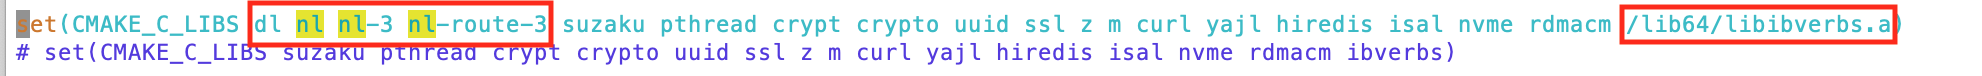
\includegraphics[width=10cm]{../imgs/cmake-link-static.png}
\end{center}

生成静态库
\begin{myeasylist}{itemize}
& SHARED  -> STATIC
& LIBRARY -> ARCHIVE
\end{myeasylist}

\section{gdb}

\begin{myeasylist}{itemize}
& ~/.gdbinit
& info registers
& info sharedlibrary
& gdb -p
\end{myeasylist}

gdb -p发现了mbuffer\_writefile进入死循环,原因是count==0。

猜想是重入了一个锁。

\section{wireshark}

\chapter{领域模型}

\chapter{核心数据结构}

\section{ETCD}

集群状态

\section{元数据管理}

对象标识和寻址机制

\section{SQLITE}

异步化

\section{DISK BITMAP}

空间分配器

\section{LEASE}

\section{CLOCK}

副本数据一致性

\section{MSGQUEUE}

离线消息处理

异步化,是否可提取出异步化框架?

\section{控制器缓存}

采用引用计数技术。

控制器切换和平衡

\section{副本缓存}

\section{扩展属性}

\section{快照}

\section{克隆卷}

\section{CORE AND Scheduler}

每个core有独立scheduler。为了与其它节点上的core进行通信,抽象出了corenet的概念。

实体标识和命名:hostname,nid,core hash,sockid。

RPC有发送端和接收端。

\chapter{关键过程}

过程分析分两种:正常情况和异常情况。特别是故障情况下,过程之间存在广泛的交互作用,变得更为复杂。

过程需要具备一些重要属性,如事务ACID,safety和liveness等,要具体情况具体分析。
值得注意的是,若干过程需要实现为可重入的。

其它注意事项:
\begin{compactenum}
\item 必须正确处理过程的返回值。
\item 一定要检查加锁的返回值,返回值失败,不能unlock,从而保证加锁解锁的对称性
\item 资源的分配和释放,使用goto方法,用stack方式管理
\item 过程运行在协程内,还是协程外?
\item 变量作用域,在作用域以外访问变量
\item 过程是否并发安全?
\item 过程执行时间是否过长,且中间无中断?比如有大循环,有同步IO操作等
\end{compactenum}

实体有复合和简单之分。简单实体的基本操作包括增删改查,复合实体在此基础上多出了子节点的相关操作。

按一颗树来组织,简单实体是叶子节点,复合实体是中间节点或根节点。

if-then/what-if假设分析:
\begin{compactenum}
\item 资源管理的对称性(分配/释放, 资源包括fd,lock,malloc等)
\item 如果此处发生故障,会如何?容错
\item 如果有多个task进入,会如何?并发
\item 会有什么不良影响吗?safety
\item 过程能完成吗?liveness
\end{compactenum}

事务分析:
\begin{compactenum}
\item 可串行化(两阶段锁,树协议)
\item 事务日志:持久化每一个操作,包括必须的上下文信息
\item 重启时,REDO/UNDO(原子性)
\item 为减少需要REDO的操作,记录检查点
\end{compactenum}

\section{集群}

\subsection{加入节点}

\subsection{删除节点}

\section{存储池}

\subsection{创建存储池}

\subsection{删除存储池}

\subsection{添加磁盘}

% \subsection{添加缓存盘}

\subsection{删除磁盘}

拔盘会产生一系列的影响,如IO抖动,控制器主副本丢失,存储池降级等。
与读写,控制器切换,QoS策略,恢复,平衡等过程都有密切关系。

\begin{compactenum}
\item 更高效的检测方法
\item 何时关闭fd,应避免fd重用造成的影响
\item 如何降低check过程对性能的干扰
\item lich health clean是否可以自动化
\item 盘会不会重新加入,从而造成副本数增多
\item RAID的影响,干扰别的盘,造成IO中断
\item rescan,不必等到下次恢复周期
\end{compactenum}

diskid字段上加索引

\subsection{空间分配}

admin维护着集群的拓扑结构。

故障域规则

分两层:副本的节点位置和副本的磁盘位置。

注意多个chunk的局部性对性能和恢复性能的影响。

\section{目录}

\section{卷}

卷属性:
\begin{lstlisting}
- 副本数
- 精简配置
- 当前链接
\end{lstlisting}

\subsection{创建卷}

\subsection{删除卷}

\subsection{加载卷}

\begin{compactenum}
\item 延迟加载table2
\item 预加载table2
\item 获取allocate属性的方式和性能
\end{compactenum}

\subsection{分配卷空间}

局部性

\subsection{unmap卷空间}

\subsection{查询卷属性}

\subsection{计算卷md5sum}

存在不能返回的情况

\subsection{resize}

扩容,不允许缩容

\subsection{rename}

前置条件:不能跨存储池

\subsection{拷贝}

两种实现方式:读写,基于快照

考虑在server端做!

可控的并发度

前置条件和后置条件

不变式

\subsection{迁移}

同池迁移,同rename

跨池迁移,前置条件

\subsection{切换卷控制器}

\begin{compactenum}
\item 源端volume\_proto是怎么回收的?
\item lease机制怎么影响本过程?
\end{compactenum}

\subsection{write}

\subsection{read}

\section{快照}

\subsection{创建快照}

\subsection{删除快照}

\subsection{回滚快照}

\subsection{克隆}

克隆卷后,需要保护其源快照。目前,克隆关系是单向的,克隆卷记录了其源快照信息,快照没有记录克隆卷的信息。

\subsection{FLATTEN}

\section{主机映射}

\section{后台任务}

\subsection{监控磁盘状态}

\subsection{恢复}

局部性

恢复性能与批量分配有关。如果连续的chunk,被分配到部分节点的部分盘上,就会影响到恢复性能。
恢复是按卷顺序扫描,调整该顺序,可以提高并行度。

删除卷

QoS,slow start

恢复要能有效处理多种故障情况,做到高效及时,QoS。

拔盘时,通过chunk\_check过程进行恢复。读发生在多个节点上,写发生在拔的盘所在节点(?)。
如果该节点盘较少,会影响到恢复性能。

\subsection{平衡}

平衡分控制器平衡和数据平衡。

卷在节点间和节点内的平衡,节点内core间平衡,可以引入一hash table来解决,
带来的问题是什么?可以容易地克服吗?

通过迁移控制器来实现卷在节点和corenet上的平衡。每个corenet指的是各个节点上具有相同core hash的core组成的网络。

平衡算法要保证输出的稳定性,分两阶段:定位和迁移。定位阶段确定所有卷控制器的位置,每个卷最多迁移一次。

\subsection{回收卷}

\subsection{回收快照}

\subsection{恢复快照}

\subsection{FLAT卷}

flat性能分析:读,分配,写多个阶段。能否批处理?并发度如何?

快照树

精简配置

删除卷

因为table2的写入特性,顺序处理各个chunk,并发度不高。

分布式并发?

属性依赖性:source < clone < flat。生成顺序是顺序的,flat完成后的重置顺序则是逆序的。
一般的事务过程,各阶段的顺序,也许按依赖性进行分析。无依赖的,理论上是可以并发的。
分布式系统的因果序,happen-before关系。

\subsection{存储池状态}

\begin{compactitem}
\item Available
\item Degraded
\item Readonly
\item Unavailable
\end{compactitem}

异步处理

cron后台执行一定的策略,如nagios等监控系统,处理结果放入/dev/shm

时间戳

pending状态

\chapter{运行时结构}

\section{CORE}

\subsection{\_\_core\_worker}

\section{磁盘管理}

\subsection{diskctl\_start}

\chapter{标准库}

\section{CPU}

\subsection{pthread}
\subsection{coroutine}

\section{Memory}

\subsection{ymalloc}
\subsection{mem\_cache}
\subsection{mbuffer}

\section{Disk}

\subsection{Local File and Directory}
\subsection{AIO}

\section{Network}

\subsection{minirpc}
\subsection{rpc}
\subsection{corerpc}

\section{String}
\section{List}
\section{Hash}
\section{Skip List}
\section{Cache with ref}
\section{Date and Time}
\section{JSON}
\section{Lease}
\section{ETCD}

\chapter{FAQ}

问题集:
\begin{enumbox}
\item /的位置信息
\item 当前分配的最大卷ID?
\end{enumbox}

P1: IOMeter测试,256K,Lich顺序和随机IO性能差别大

P2: lsv\_gc\_check断言失败

P3: Error Handling


\end{document}
